\documentclass[twoside]{book}

% Packages required by doxygen
\usepackage{fixltx2e}
\usepackage{calc}
\usepackage{doxygen}
\usepackage{graphicx}
\usepackage[utf8]{inputenc}
\usepackage{makeidx}
\usepackage{multicol}
\usepackage{multirow}
\PassOptionsToPackage{warn}{textcomp}
\usepackage{textcomp}
\usepackage[nointegrals]{wasysym}
\usepackage[table]{xcolor}

% Font selection
\usepackage[T1]{fontenc}
\usepackage{mathptmx}
\usepackage[scaled=.90]{helvet}
\usepackage{courier}
\usepackage{amssymb}
\usepackage{sectsty}
\renewcommand{\familydefault}{\sfdefault}
\allsectionsfont{%
  \fontseries{bc}\selectfont%
  \color{darkgray}%
}
\renewcommand{\DoxyLabelFont}{%
  \fontseries{bc}\selectfont%
  \color{darkgray}%
}
\newcommand{\+}{\discretionary{\mbox{\scriptsize$\hookleftarrow$}}{}{}}

% Page & text layout
\usepackage{geometry}
\geometry{%
  a4paper,%
  top=2.5cm,%
  bottom=2.5cm,%
  left=2.5cm,%
  right=2.5cm%
}
\tolerance=750
\hfuzz=15pt
\hbadness=750
\setlength{\emergencystretch}{15pt}
\setlength{\parindent}{0cm}
\setlength{\parskip}{0.2cm}
\makeatletter
\renewcommand{\paragraph}{%
  \@startsection{paragraph}{4}{0ex}{-1.0ex}{1.0ex}{%
    \normalfont\normalsize\bfseries\SS@parafont%
  }%
}
\renewcommand{\subparagraph}{%
  \@startsection{subparagraph}{5}{0ex}{-1.0ex}{1.0ex}{%
    \normalfont\normalsize\bfseries\SS@subparafont%
  }%
}
\makeatother

% Headers & footers
\usepackage{fancyhdr}
\pagestyle{fancyplain}
\fancyhead[LE]{\fancyplain{}{\bfseries\thepage}}
\fancyhead[CE]{\fancyplain{}{}}
\fancyhead[RE]{\fancyplain{}{\bfseries\leftmark}}
\fancyhead[LO]{\fancyplain{}{\bfseries\rightmark}}
\fancyhead[CO]{\fancyplain{}{}}
\fancyhead[RO]{\fancyplain{}{\bfseries\thepage}}
\fancyfoot[LE]{\fancyplain{}{}}
\fancyfoot[CE]{\fancyplain{}{}}
\fancyfoot[RE]{\fancyplain{}{\bfseries\scriptsize Generated on Thu Dec 1 2016 21\+:11\+:54 for Proyecto2 by Doxygen }}
\fancyfoot[LO]{\fancyplain{}{\bfseries\scriptsize Generated on Thu Dec 1 2016 21\+:11\+:54 for Proyecto2 by Doxygen }}
\fancyfoot[CO]{\fancyplain{}{}}
\fancyfoot[RO]{\fancyplain{}{}}
\renewcommand{\footrulewidth}{0.4pt}
\renewcommand{\chaptermark}[1]{%
  \markboth{#1}{}%
}
\renewcommand{\sectionmark}[1]{%
  \markright{\thesection\ #1}%
}

% Indices & bibliography
\usepackage{natbib}
\usepackage[titles]{tocloft}
\setcounter{tocdepth}{3}
\setcounter{secnumdepth}{5}
\makeindex

% Hyperlinks (required, but should be loaded last)
\usepackage{ifpdf}
\ifpdf
  \usepackage[pdftex,pagebackref=true]{hyperref}
\else
  \usepackage[ps2pdf,pagebackref=true]{hyperref}
\fi
\hypersetup{%
  colorlinks=true,%
  linkcolor=blue,%
  citecolor=blue,%
  unicode%
}

% Custom commands
\newcommand{\clearemptydoublepage}{%
  \newpage{\pagestyle{empty}\cleardoublepage}%
}


%===== C O N T E N T S =====

\begin{document}

% Titlepage & ToC
\hypersetup{pageanchor=false,
             bookmarks=true,
             bookmarksnumbered=true,
             pdfencoding=unicode
            }
\pagenumbering{roman}
\begin{titlepage}
\vspace*{7cm}
\begin{center}%
{\Large Proyecto2 }\\
\vspace*{1cm}
{\large Generated by Doxygen 1.8.8}\\
\vspace*{0.5cm}
{\small Thu Dec 1 2016 21:11:54}\\
\end{center}
\end{titlepage}
\clearemptydoublepage
\tableofcontents
\clearemptydoublepage
\pagenumbering{arabic}
\hypersetup{pageanchor=true}

%--- Begin generated contents ---
\chapter{Class Index}
\section{Class List}
Here are the classes, structs, unions and interfaces with brief descriptions\+:\begin{DoxyCompactList}
\item\contentsline{section}{\hyperlink{class_juego_de_la_vida}{Juego\+De\+La\+Vida} }{\pageref{class_juego_de_la_vida}}{}
\end{DoxyCompactList}

\chapter{Class Documentation}
\hypertarget{class_astar}{\section{Astar Class Reference}
\label{class_astar}\index{Astar@{Astar}}
}


Collaboration diagram for Astar\+:
\nopagebreak
\begin{figure}[H]
\begin{center}
\leavevmode
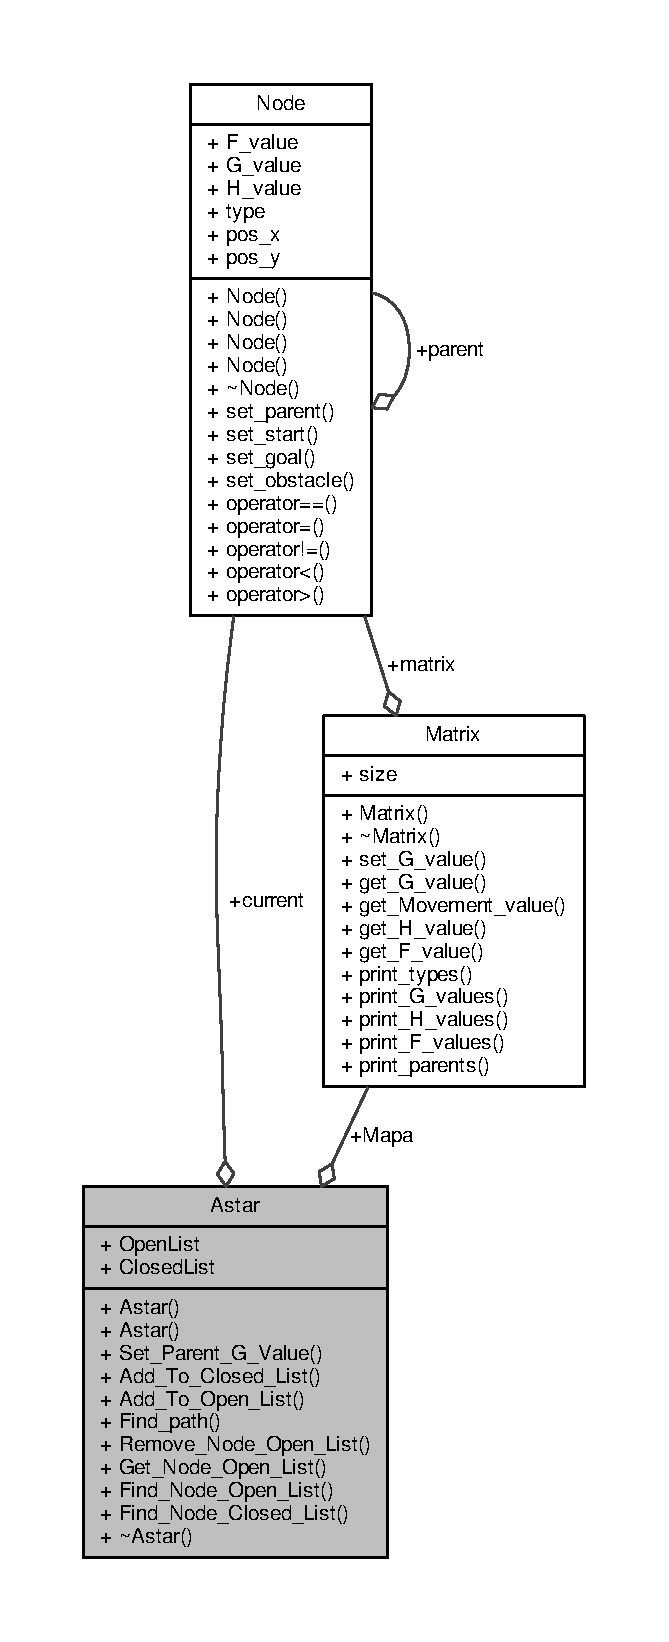
\includegraphics[height=550pt]{class_astar__coll__graph}
\end{center}
\end{figure}
\subsection*{Public Member Functions}
\begin{DoxyCompactItemize}
\item 
\hypertarget{class_astar_aefad6a17cda946cd45c5e5027489934b}{{\bfseries Astar} (int tam, int start\+\_\+x, int start\+\_\+y, int goal\+\_\+x, int goal\+\_\+y)}\label{class_astar_aefad6a17cda946cd45c5e5027489934b}

\item 
\hypertarget{class_astar_a52886c312f2f7b27aed52843768cf8c2}{void {\bfseries Set\+\_\+\+Parent\+\_\+\+G\+\_\+\+Value} (\hyperlink{class_node}{Node} actual)}\label{class_astar_a52886c312f2f7b27aed52843768cf8c2}

\item 
\hypertarget{class_astar_ab748b97eb928002c29259b1c9a3d7347}{void {\bfseries Add\+\_\+\+To\+\_\+\+Closed\+\_\+\+List} (\hyperlink{class_node}{Node} actual)}\label{class_astar_ab748b97eb928002c29259b1c9a3d7347}

\item 
\hypertarget{class_astar_a27e5c51c01c59b6a2a8b940d86803a14}{void {\bfseries Add\+\_\+\+To\+\_\+\+Open\+\_\+\+List} (\hyperlink{class_node}{Node} actual)}\label{class_astar_a27e5c51c01c59b6a2a8b940d86803a14}

\item 
\hypertarget{class_astar_a65758f9edc318accb69162dde384b970}{void {\bfseries Find\+\_\+path} (\hyperlink{class_node}{Node} \&current)}\label{class_astar_a65758f9edc318accb69162dde384b970}

\item 
\hypertarget{class_astar_aa8a2361e27946f15951cbc64d194aeb0}{void {\bfseries Remove\+\_\+\+Node\+\_\+\+Open\+\_\+\+List} ()}\label{class_astar_aa8a2361e27946f15951cbc64d194aeb0}

\item 
\hypertarget{class_astar_a5b6e55b61c0ab7a61ddb34cad145cf8e}{\hyperlink{class_node}{Node} {\bfseries Get\+\_\+\+Node\+\_\+\+Open\+\_\+\+List} ()}\label{class_astar_a5b6e55b61c0ab7a61ddb34cad145cf8e}

\item 
\hypertarget{class_astar_a99b6a25688450de001e23aabe1068058}{int {\bfseries Find\+\_\+\+Node\+\_\+\+Open\+\_\+\+List} (const \hyperlink{class_node}{Node} a)}\label{class_astar_a99b6a25688450de001e23aabe1068058}

\item 
\hypertarget{class_astar_a2f540a660bbc37fb6fb092d65a9485d5}{int {\bfseries Find\+\_\+\+Node\+\_\+\+Closed\+\_\+\+List} (const \hyperlink{class_node}{Node} b)}\label{class_astar_a2f540a660bbc37fb6fb092d65a9485d5}

\end{DoxyCompactItemize}
\subsection*{Public Attributes}
\begin{DoxyCompactItemize}
\item 
\hypertarget{class_astar_a318fbaf1e03319281b454caac6710361}{vector$<$ \hyperlink{class_node}{Node} $>$ {\bfseries Open\+List}}\label{class_astar_a318fbaf1e03319281b454caac6710361}

\item 
\hypertarget{class_astar_a6b15d8a00431db17af288977ee4b9fca}{vector$<$ \hyperlink{class_node}{Node} $>$ {\bfseries Closed\+List}}\label{class_astar_a6b15d8a00431db17af288977ee4b9fca}

\item 
\hypertarget{class_astar_a5d1206b313064705051e9c2607afad94}{\hyperlink{class_matrix}{Matrix} $\ast$ {\bfseries Mapa}}\label{class_astar_a5d1206b313064705051e9c2607afad94}

\item 
\hypertarget{class_astar_a943695a46f99f1617891efdab1a5d9c7}{\hyperlink{class_node}{Node} {\bfseries current}}\label{class_astar_a943695a46f99f1617891efdab1a5d9c7}

\end{DoxyCompactItemize}


The documentation for this class was generated from the following files\+:\begin{DoxyCompactItemize}
\item 
Astar.\+h\item 
Astar.\+cpp\end{DoxyCompactItemize}

\hypertarget{class_matrix}{\section{Matrix Class Reference}
\label{class_matrix}\index{Matrix@{Matrix}}
}


Collaboration diagram for Matrix\+:
\nopagebreak
\begin{figure}[H]
\begin{center}
\leavevmode
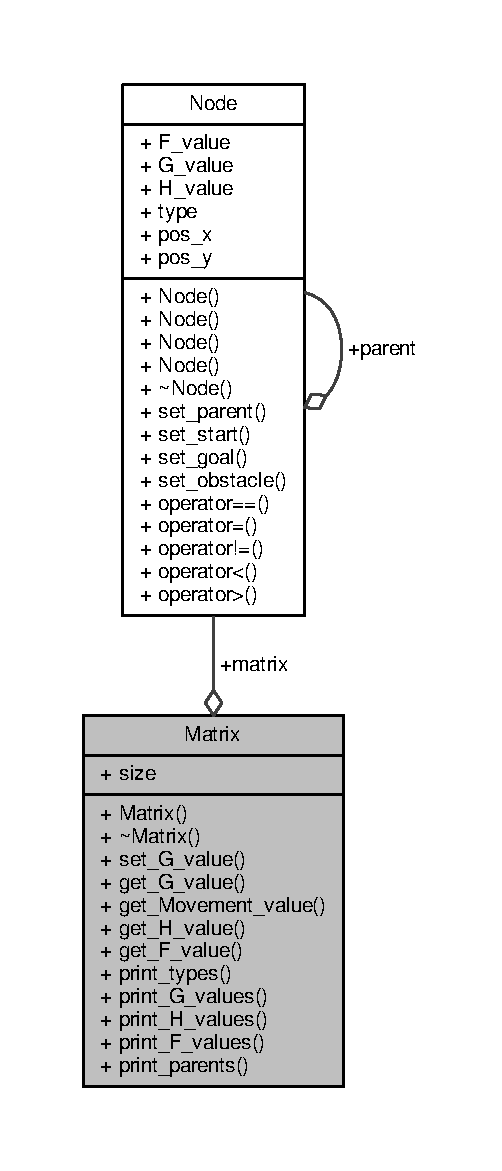
\includegraphics[width=196pt]{class_matrix__coll__graph}
\end{center}
\end{figure}
\subsection*{Public Member Functions}
\begin{DoxyCompactItemize}
\item 
\hypertarget{class_matrix_ae763d5a5d65e3c0f185bebd7766124ba}{{\bfseries Matrix} (int tam)}\label{class_matrix_ae763d5a5d65e3c0f185bebd7766124ba}

\item 
\hypertarget{class_matrix_ae1235f5c15ae98654e92ea2661ca60ea}{{\bfseries Matrix} (int $\ast$$\ast$values, int tam)}\label{class_matrix_ae1235f5c15ae98654e92ea2661ca60ea}

\item 
\hypertarget{class_matrix_a1e9a500f0ca4e681153fee9b2727b836}{void {\bfseries change\+\_\+size} (int new\+\_\+size)}\label{class_matrix_a1e9a500f0ca4e681153fee9b2727b836}

\item 
\hypertarget{class_matrix_a8360b94a374a116db0cc9163467ac4d7}{void {\bfseries remove\+\_\+rowcolumn} (int row)}\label{class_matrix_a8360b94a374a116db0cc9163467ac4d7}

\item 
\hypertarget{class_matrix_a63682775de6a8d35bc89cabbc35e2d61}{int $\ast$ {\bfseries find\+\_\+edge} (int e)}\label{class_matrix_a63682775de6a8d35bc89cabbc35e2d61}

\item 
\hypertarget{class_matrix_a99ba97122b8fdd54e95290caf80fc8e2}{void {\bfseries print} ()}\label{class_matrix_a99ba97122b8fdd54e95290caf80fc8e2}

\end{DoxyCompactItemize}
\subsection*{Public Attributes}
\begin{DoxyCompactItemize}
\item 
\hypertarget{class_matrix_a0df8ee2a361c4d678fcde2fcf3a8e4f9}{int $\ast$$\ast$ {\bfseries matrix}}\label{class_matrix_a0df8ee2a361c4d678fcde2fcf3a8e4f9}

\item 
\hypertarget{class_matrix_acd4947d87d17f777df33e32cef2e873c}{int {\bfseries size}}\label{class_matrix_acd4947d87d17f777df33e32cef2e873c}

\end{DoxyCompactItemize}


The documentation for this class was generated from the following files\+:\begin{DoxyCompactItemize}
\item 
Matrix.\+h\item 
Matrix.\+cpp\end{DoxyCompactItemize}

\hypertarget{class_node}{\section{Node Class Reference}
\label{class_node}\index{Node@{Node}}
}


Collaboration diagram for Node\+:
\nopagebreak
\begin{figure}[H]
\begin{center}
\leavevmode
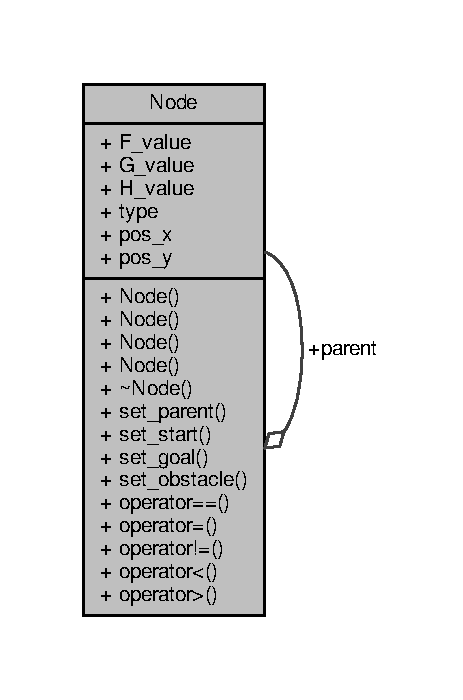
\includegraphics[width=222pt]{class_node__coll__graph}
\end{center}
\end{figure}
\subsection*{Public Member Functions}
\begin{DoxyCompactItemize}
\item 
\hypertarget{class_node_a7c677bda3076d3d8eccdf7831e862ac2}{{\bfseries Node} (const \hyperlink{class_node}{Node} \&N)}\label{class_node_a7c677bda3076d3d8eccdf7831e862ac2}

\item 
\hypertarget{class_node_a23a19f53dfbb18fec58cdac90de3d144}{{\bfseries Node} (int x, int y)}\label{class_node_a23a19f53dfbb18fec58cdac90de3d144}

\item 
\hypertarget{class_node_af1d32d3c0489e11f081ff36db1394e12}{{\bfseries Node} (int f, int g, int h, int type, \hyperlink{class_node}{Node} $\ast$father)}\label{class_node_af1d32d3c0489e11f081ff36db1394e12}

\item 
\hypertarget{class_node_acfef82742f32525c7b62a6fb99f533c2}{void {\bfseries set\+\_\+parent} (\hyperlink{class_node}{Node} p)}\label{class_node_acfef82742f32525c7b62a6fb99f533c2}

\item 
\hypertarget{class_node_a05b14800e32cabc3631c4e74c09d6ad6}{void {\bfseries set\+\_\+start} ()}\label{class_node_a05b14800e32cabc3631c4e74c09d6ad6}

\item 
\hypertarget{class_node_ad92eea96378329a57cbd2a867e883119}{void {\bfseries set\+\_\+goal} ()}\label{class_node_ad92eea96378329a57cbd2a867e883119}

\item 
\hypertarget{class_node_ab7860d8fd548624055e04e4152233fc1}{void {\bfseries set\+\_\+obstacle} ()}\label{class_node_ab7860d8fd548624055e04e4152233fc1}

\item 
\hypertarget{class_node_ac38b044237716c27fc53d55984919569}{int {\bfseries operator==} (const \hyperlink{class_node}{Node} \&N) const }\label{class_node_ac38b044237716c27fc53d55984919569}

\item 
\hypertarget{class_node_aac90c7101fc00cb58eb15b8657bbf392}{\hyperlink{class_node}{Node} \& {\bfseries operator=} (const \hyperlink{class_node}{Node} \&N)}\label{class_node_aac90c7101fc00cb58eb15b8657bbf392}

\item 
\hypertarget{class_node_a3c2cd5ef2f31b2742c65b6a5321d2ca8}{int {\bfseries operator!=} (const \hyperlink{class_node}{Node} \&N) const }\label{class_node_a3c2cd5ef2f31b2742c65b6a5321d2ca8}

\item 
\hypertarget{class_node_a6df353aa334e4273d90889aed8d2762b}{int {\bfseries operator$<$} (const \hyperlink{class_node}{Node} \&N) const }\label{class_node_a6df353aa334e4273d90889aed8d2762b}

\item 
\hypertarget{class_node_a5b3a60439297eff107faf6de1b5fc53a}{int {\bfseries operator$>$} (const \hyperlink{class_node}{Node} \&N) const }\label{class_node_a5b3a60439297eff107faf6de1b5fc53a}

\end{DoxyCompactItemize}
\subsection*{Public Attributes}
\begin{DoxyCompactItemize}
\item 
\hypertarget{class_node_abaac411cb792ada4aafd40f09cbbfeb3}{int {\bfseries F\+\_\+value}}\label{class_node_abaac411cb792ada4aafd40f09cbbfeb3}

\item 
\hypertarget{class_node_a204590a559408957a9828cb731be0262}{int {\bfseries G\+\_\+value}}\label{class_node_a204590a559408957a9828cb731be0262}

\item 
\hypertarget{class_node_a5fd0078658a5b48f612b7dc6edd9e4b2}{int {\bfseries H\+\_\+value}}\label{class_node_a5fd0078658a5b48f612b7dc6edd9e4b2}

\item 
\hypertarget{class_node_a86fcc8384153457dcc9bcaf65c8fbec3}{int {\bfseries type}}\label{class_node_a86fcc8384153457dcc9bcaf65c8fbec3}

\item 
\hypertarget{class_node_ad8184598cdea70e4bbdfd76f2b0f9e85}{\hyperlink{class_node}{Node} $\ast$ \hyperlink{class_node_ad8184598cdea70e4bbdfd76f2b0f9e85}{parent}}\label{class_node_ad8184598cdea70e4bbdfd76f2b0f9e85}

\begin{DoxyCompactList}\small\item\em 0 para nodo normal,1 para start, 2 para goal, 3 para obstaculo y 4 para path \end{DoxyCompactList}\item 
\hypertarget{class_node_a5fb3136718750eac5a24802ca095fd71}{int {\bfseries pos\+\_\+x}}\label{class_node_a5fb3136718750eac5a24802ca095fd71}

\item 
\hypertarget{class_node_ad53bede56c310225b514c8539f61077e}{int {\bfseries pos\+\_\+y}}\label{class_node_ad53bede56c310225b514c8539f61077e}

\end{DoxyCompactItemize}


The documentation for this class was generated from the following files\+:\begin{DoxyCompactItemize}
\item 
Node.\+h\item 
Node.\+cpp\end{DoxyCompactItemize}

%--- End generated contents ---

% Index
\newpage
\phantomsection
\addcontentsline{toc}{chapter}{Index}
\printindex

\end{document}
